\phantomsection

\chapter{State of the art}
\markboth{State of the art}{}

\begin{citazione}
\end{citazione}
\newpage

\section{Denial of Service detection techniques}
Since Denial of Service attacks have always been a crucial threat to Data Centers security, over the years researchers carried out several studies about \emph{DoS} detection techniques. Most of these techniques rely on the use of Intrusion Detection Systems \emph{(IDS)} implementing detection mechanisms mostly based on Artificial Intelligence techniques. This section summarizes some of the research works about this topic available in literature:
\begin{itemize}
\item \emph{Wei Zhou et al.} \cite{zhou2014detection} proposed a method to detect Application Layer Distributed Denial of Service (\emph{AL-DDoS}) attacks in heavy backbone traffic. This approach models the traffic in real-time and, through an examination of the entropy of AL-DDoS attacks and flash crowds (i.e. the legitimate traffic), it is capable to distinguish between these two cases and detect real \emph{AL-DDoS} attacks. The authors tested this algorithm on real data and claimed it is effective to identify and stop attack sources. However they mentioned the need to improve the reaction rate leaving it as a possible future development;
\item \emph{JaehakYu et al.} \cite{yu2008traffic} proposed a lightweight detection algorithm for \emph{DoS} that collects statistical information from \emph{Simple Network Management Protocol (SNMP)} agents instead of analyzing raw packet data. This approach, combined with the machine learning technique based on a \emph{Support Vector Machine (SVM)} for attack classification, resulted in rapid detection and high accuracy;
\item \emph{Ming-hui Yang et al.} \cite{yang2008ddos} improved \emph{SVM} detection technique, introducing an approach that combined \emph{SVM} and the wavelet kernel function (i.e. a multidimensional wavelet function that can approximate arbitrary nonlinear functions \cite{zhang2004wavelet}) theory, achieving an improvement of 4\% compared to the traditional \emph{SVM} approach. 
\item \emph{T. Spyridopoulos et al.} \cite{spyridopoulos2013game} proposed a game-theoretic approach to \emph{DDoS} attack detection where the \emph{DDoS} attack is modeled as a one-shot non-cooperative, zero-sum game. By analyzing several parameters such as the cost to perform the attack, the number of attacking nodes and malicious traffic probability distributions, authors were able to identify the only optimal strategy available to the defender under the hypothesis that the attacker is a rational player. 
\item \emph{Uğur Akyazı et al.} \cite{akyazi2010detection} capitalized on the similarity between the architecture of \emph{IDS} and the Biological Immune Systems, developing an Artificial Immune System as a method of anomaly-based \emph{IDS}. Their algorithm achieved high accuracy and precision under certain parameters and experimental conditions described in the forementioned paper;
\item \emph{Wanchun Dou et al.} \cite{dou2013confidence} proposed a real-time Confidence-Based Filtering method as a \emph{DDoS} defending approach. This approach collects packets from non-attacking periods in order to generate a nominal traffic profile that is used to calculate the score of packets in the attack period. This score indicates whether to discard or not a certain packet. Authors claimed that the proposed algorithm has a high scoring speed, a small storage requirement and an acceptable filtering accuracy;
\item \emph{Mehdi Barati et al.} \cite{barati2014distributed} proposed a detection architecture that uses a Genetic Algorithm for feature selection and an Artificial Neural Network for attack detection. High accuracy and deniable false alarm have been achieved by this algorithm. 
\end{itemize}
\section{Simulation tools comparison} { \setstretch{1.3}
Simulation tools play a critical role in various domains of cloud computing. They offer researchers and infrastructure designers a virtual environment to work in, eliminating the expenses associated with physical infrastructure. Over time, several authors have conducted comparative studies to assess different simulators and highlight their unique characteristics, assisting users in selecting the most suitable option for their specific context. In this section, several cloud simulators that have been studied by the researchers will be discussed, focusing on their main strengths, drawbacks and the problems they aim to address. Since the main focus is to identify a simulator that is well-suited for energy consumption metrics extraction, features that ensure the accuracy of the simulations will be prioritized in order to make this work relevant in real scenarios. The following argument is based on several previous surveys, namely: \emph{N. Mansouri, et al.} \cite{mansouri2020cloud}, \emph{P. Suryateja} \cite{suryateja2016comparative}, \emph{D. Perez Abreu, et al.} \cite{abreu2020comparative}, \emph{Khaled M. Khalil, et al.} \cite{khalil2017cloud}, \emph{Nimisha Patel
\& Hiren Patel} \cite{patel2016comprehensive}.
 
\subsubsection{CloudSim}
When it comes to cloud simulators it is impossible to overlook \emph{CloudSim} \cite{calheiros2011cloudsim}, as it is one of the most widely used \emph{event-driven} tools among researchers. A search for the keyword "\emph{CloudSim}" on the \emph{Scopus} platform yields 2020 results (this search was performed in May 2023), indicating its widespread adoption in the research community. Over the years, several simulators based on \emph{CloudSim} have been proposed. This tool, written in \emph{Java}, is comprehensive and highly extensible.
One notable feature is its virtualization engine, which allows the creation and management of virtualization services on a network node. Additionally, \emph{CloudSim} provides the capability to allocate machine cores in two different ways: space-shared and time-shared.
In space-shared allocation, each machine is divided into a set of cores, and each core is assigned to a single job until it is completed. On the other hand, in time-shared allocation multiple jobs can be assigned to a single core and each of them is executed for a certain amount of time before another job is chosen.
Overall, \emph{CloudSim} offers researchers a comprehensive and flexible platform to simulate and study virtualization and resource allocation techniques \cite{mansouri2020cloud}.
Architecture of \emph{CloudSim} is shown in figure \ref{fig:cloudsim_arch}. It is composed by three layers, described below:
\begin{itemize}
    \item \textbf{CloudSim core simulation engine}: initially implemented through the discrete event simulation engine \emph{SimJava} that supports functionalities such as queuing, processing of events, creation of Cloud system entities, communication between components and management of the simulation clock (\cite{calheiros2011cloudsim}), it has been replaced with an engine that provides some advanced operations;
    \item \textbf{CloudSim simulation level}: it provides various interfaces and services that allow to model and simulate Cloud-based data center environments; 
    \item \textbf{User code}: it allows to set up various simulation parameters such as number of machines, their specification, number of tasks and broker scheduling policies.
\end{itemize}
\begin{figure}[h]
    \centering
    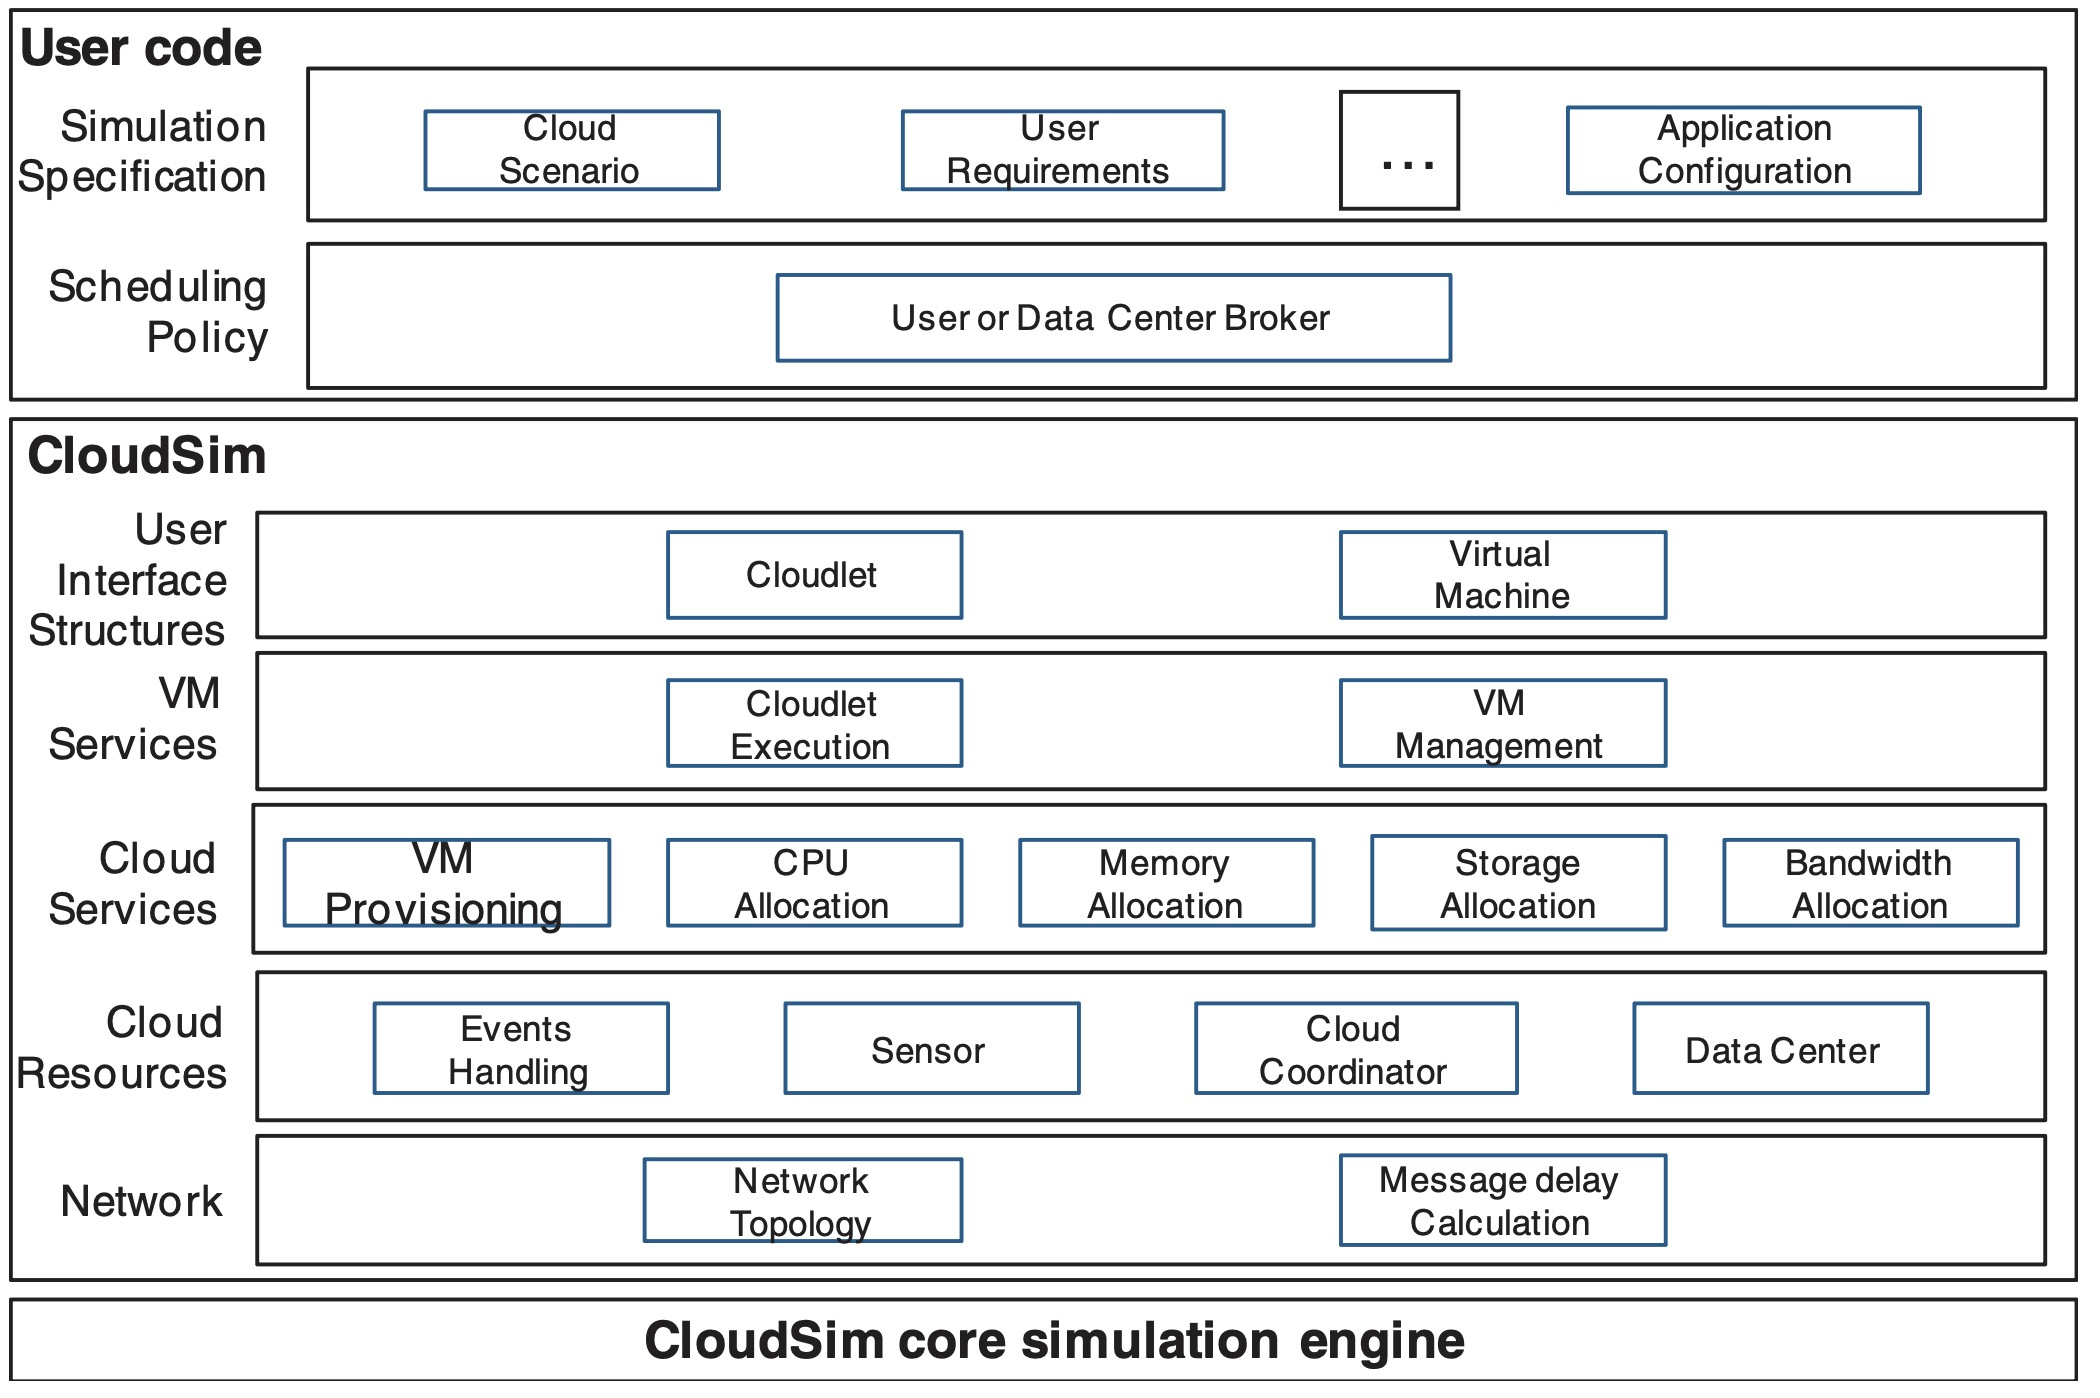
\includegraphics[width=0.5\textwidth]{chapters/images/cloudsim_arch.jpeg}
    \caption{CloudSim architecture}
    \label{fig:cloudsim_arch}
\end{figure}
\subsubsection{NetworkCloudSim}
\emph{NetworkCloudSim} \cite{garg2011networkcloudsim} implements a network layer and  provides several communication models, including message-based, packet-based and flow-based models. It also offers an accurate evaluation of the scheduling of machines in the data center. Finally, it provides a basic energy model of the data center, although it does not extensively focus on energy efficiency and it does not provide a packet-level network model \cite{mansouri2020cloud} \cite{patel2016comprehensive}.
\subsubsection*{CloudAnalyst}
\emph{CloudAnalyst} \cite{wickremasinghe2010cloudanalyst} makes simulation work easier as it provides a \emph{GUI}. Its main features is the ability to gather information about the geographical location of users and data centers. The simulator also offers a set of metrics based on response time and request processing. However, it does not implement a complete communication model based on the \emph{TCP/IP} protocol and it provides a poor energy model \cite{mansouri2020cloud}. 
\subsubsection{EMUSim}
\emph{EMUSim} \cite{calheiros2013emusim} includes an emulation and a simulation environment. The simulator is able to get profiling data about the running application behavior through the emulation environment; these data are used to build a simulation environment. However, the emulation environment strongly limits scalability and makes the simulator not suitable for large workload scenarios \cite{mansouri2020cloud}. 
\subsubsection*{CDOSim}
\emph{CDOSim} \cite{fittkau2012cdosim} integrates \emph{CloudSim} simulator and \emph{CloudMIG} framework. This simulator adopts a scaling technique that assigns a new virtual machine when CPU usage exceeds a specific threshold.  It provides a set of client-centric metrics, allowing developers to compare different solutions based on various deployment parameters. Another noteworthy feature is the presence of a benchmark module that detects the impact of choosing a specific architecture on application performance. However, the communication model employed by CDOSim is overly simplistic and strongly limits large-scale applications \cite{mansouri2020cloud}.
\subsubsection*{TeachCloud}
\emph{TeachCloud} \cite{jararweh2013teachcloud} is designed to be suitable for students who want to have some practical experience with Cloud Computing simulation, covering aspects such as networking, Service Level Agreement contraints, web-based applications, Service Oriented Architecture, virtualization, and so on. Through a user-friendly \emph{GUI} it allows to design several network architectures in addition to the pre-existing ones. This simulator lacks realism in various aspects since it is mainly designed for academic purposes. For example, the simulator does not consider the possibility of faults in the data center, preventing developers from studying the impact of faults on application usage \cite{mansouri2020cloud} \cite{patel2016comprehensive}.
\subsubsection*{DartCSim}
\emph{DartCSim} \cite{li2012dartcsim} provides a simple \emph{GUI} that allows users to set various simulation parameters, such as the characteristics of the data center and the network topology. These parameters can be imported and exported at any level of the simulation and can be set for individual CPUs or the entire data center. However, this tool lacks a comprehensive energy model, which prevents developers from implementing strategies aimed at improving data center efficiency \cite{mansouri2020cloud}.
\subsubsection*{DartCSim+}
\emph{DartCSim+} \cite{li2013dartcsim+} aims to enhance \emph{CloudSim} by introducing an energy model and a network model, allowing developers to design power-aware scheduling algorithms. However, this simulator does not include a cost model and lacks security features, which prevents developers from analyzing the security aspects of the data center \cite{mansouri2020cloud}.
\subsubsection*{ElasticSim}
\emph{ElasticSim}'s \cite{cai2017elasticsim} main feature is the resources runtime auto-scaling based on stochastic modeling that allows developers to design efficient scheduling algorithms. However, this simulator provides a poor energy consumption model and it cannot simulate security-related experiments. \cite{mansouri2020cloud}
\subsubsection*{FederatedCloudSim}
\emph{FederatedCloudSim} \cite{kohne2014federatedcloudsim} provides developers with the capability to test several types of cloud federations; this simulator is built upon the functionalities of \emph{CloudSim} and expands them by incorporating Service Level Agreement management, workload generation, event logging, scheduling, and brokering. While the simulator offers comprehensive functionality for modeling and simulating cloud federations, it does not provide specific insights into the energy consumption of each data center in the federation \cite{mansouri2020cloud}.
\subsubsection*{FTCloudSim}
\emph{FTCloudSim} \cite{zhou2013ftcloudsim} is primarily designed to simulate reliability mechanisms in cloud services. It offers implementations of various reliability mechanisms, allowing developers to analyze and evaluate the performance of these mechanisms. The simulator also includes fault generation services, which enable the generation of faults based on specific probability distributions. However, one drawback of FTCloudSim is its simplified energy consumption model, which can impact the assessment of energy-efficient strategies or algorithms \cite{mansouri2020cloud}.
\subsubsection*{WorkflowSim}
\emph{WorkflowSim} \cite{chen2012workflowsim} provides a platform for studying the performance impact of different job clustering strategies in a data center. It achieves this by implementing various workflow scheduling methods. However, WorkflowSim has limitations when it comes to simulating data-intensive applications. It does not consider the delays caused by input-output operations, which are crucial in such scenarios. Additionally, the supported fault model in WorkflowSim is limited, which can affect the realism of simulations. As a result, the accuracy and realism of simulations involving data-intensive applications may be compromised \cite{mansouri2020cloud}. 
\subsubsection*{CloudReports}
\emph{CloudReports} \cite{teixeira2014cloudreports} provides developers with a user-friendly \emph{GUI} that allows them to manage various aspects of the data center and access detailed reports on resource utilization, virtual machine allocation, and energy consumption. Since the simulator offers valuable insights into these metrics, it enables developers to optimize resource usage and energy efficiency.
On the other hand, one limitation of \emph{CloudReports} is the absence of a security layer: this means that developers cannot explore and evaluate the security characteristics of the data center using this simulator \cite{mansouri2020cloud}.
\subsubsection*{CEPSim}
\emph{CEPSim} \cite{higashino2015cepsim} models various \emph{Complex Event Processing (CEP)} environments \cite{luckham1998complex} where users can define queries using different proprietary languages and model the execution flow using a directed acyclic graph. The simulator implements various load scheduling algorithms, allowing developers to evaluate queries under different load conditions. However, one limitation of \emph{CEPSim} is that it does not consider network consumption. As a result, the simulator may not provide a comprehensive analysis of energy consumption from a network perspective. Other factors such as network transmission impact on energy consumption are not explicitly taken into account \cite{mansouri2020cloud}.
\subsubsection*{DynamicCloudSim}
\emph{DynamicCloudSim} \cite{bux2013dynamiccloudsim} is primarily concerned with addressing the instability of computing center parameters that can change during runtime. It specifically introduces failure models for task execution, allowing developers to define the failure rate when conducting experiments in a simulated environment. However, one limitation is that developers do not have the capability to calculate the energy consumption of the experiments accurately due to the restricted nature of the provided energy model; moreover, its failure model is strongly limited. \cite{mansouri2020cloud} \cite{suryateja2016comparative}
\subsubsection*{CloudExp}
\emph{CloudExp} \cite{jararweh2014cloudexp} provides developers with a simple \emph{GUI} that allows easy configuration of environment parameters and monitoring of their behavior. Specifically, CloudExp enables the definition of a Service Level Agreement (SLA) based on parameters such as the number of users, service availability and cost, network performance, and security measures. Additionally, it establishes a specialized framework for cloud computing in mobile device scenarios. However, the energy model used by the simulator is simplistic and not suitable for analyzing energy-aware strategies \cite{mansouri2020cloud} \cite{khalil2017cloud}.
\subsubsection*{CM Cloud}
\emph{CM Cloud} \cite{alves2016cm} is able to estimate overall energy simulation expenses through a comparison between several providers such as \emph{Google}, \emph{Microsoft} and \emph{Amazon}. However, this simulator lacks a complete communication model, not allowing developers to define specific traffic patterns or investigate the overall impact of the traffic generated by the hosts of the network. Finally, there is no task failure model \cite{mansouri2020cloud}.
\subsubsection*{MR-CloudSim}
\emph{MR-CloudSim} \cite{jung2012mr} is based on the \emph{MapReduce} computational model \cite{dean2008mapreduce} for big data computation, allowing developers to work with data-intensive applications. One limitation is that it does not allow developers to accurately calculate service usage expenses as it does not consider file processing time and cost \cite{mansouri2020cloud}.
\subsubsection*{UCloud}
\emph{UCloud} \cite{sqalli2012ucloud} is designed to address educational purposes as it simulates cloud for universities, allowing developers to evaluate several policies in the public and private clouds. However, this simulator lacks a support for security policies and a cost model. \cite{mansouri2020cloud}
\subsubsection*{CloudSimSDN}
\emph{CloudSimSDN} \cite{son2015cloudsimsdn} is built for cloud environments based on \emph{Software Defined Networking}, namely a programmatic approach to network management \cite{benzekki2016software}. It is a scalable simulator that allows to manage energy consumption and resource policies as well as investigate several metrics such as performance. Its major drawback is that it models applications through a set of tasks and assumes long packet transmission between VMs, which can impact the granularity of application communication, making it not well-suited for works based on applications. \cite{khalil2017cloud} \cite{abreu2020comparative}
\subsubsection*{MDCSim}
\emph{MDCSim} \cite{lim2009mdcsim} is a simulation platform for multilayer data centers analysis that allows developers to investigate applications performance under different loads and tier configurations as it has low simulation overhead. \emph{MDCSim} is able to estimate several parameters, such as throughput, response time and power consumption, so developers can compare different energy policies. However, it lacks simulation realism as it does not provide a complete network model \cite{mansouri2020cloud} \cite{patel2016comprehensive}.
\subsubsection*{GDCSim}
\emph{GDCSim} \cite{gupta2011gdcsim} is an open source, event-based simulator written in \emph{C, C++ and Shell}, as part of the \emph{BlueTool} computer infrastructure project funded by \emph{NSF}. It is designed to analyze green data centers as it provides a simulation environment where it is possible to analyze the energy consumption of the data center in a simple and accurate way. This tool also takes into account the thermal impact of the data center, giving developers the ability to design cooling policies and energy management strategies with a particular attention to the Computational Fluid Dynamics (CFD) that allows to characterize the thermal effects and airflow patterns. However, this simulator does not consider aspects related to the security of the data center. Moreover it does not allow parallel execution of defined experiments \cite{mansouri2020cloud}.
Architecture of \emph{GDCSim} is shown in figure \ref{fig:gdcsim_arch}. It is composed by four modules:
\begin{enumerate}
    \item \textbf{BlueSim Tool}: a simulation package which integrates various software for HRMs (heat recirculation matrix) array generation;
    \item \textbf{Input/Output Management}: the interface between the user and the simulator. It takes the following inputs: job trace, Service Level Agreement, management schemes and queuing model;
    \item \textbf{Resource Management}: module that implements the following algorithms: workload management, power management, cooling management and coordinated workload, power and cooling management;
    \item \textbf{Simulator}: it provides several modules such as the queuing module, the power module, the thermodynamic module and the cooling module.
\end{enumerate}
\begin{figure}[h]
    \centering
    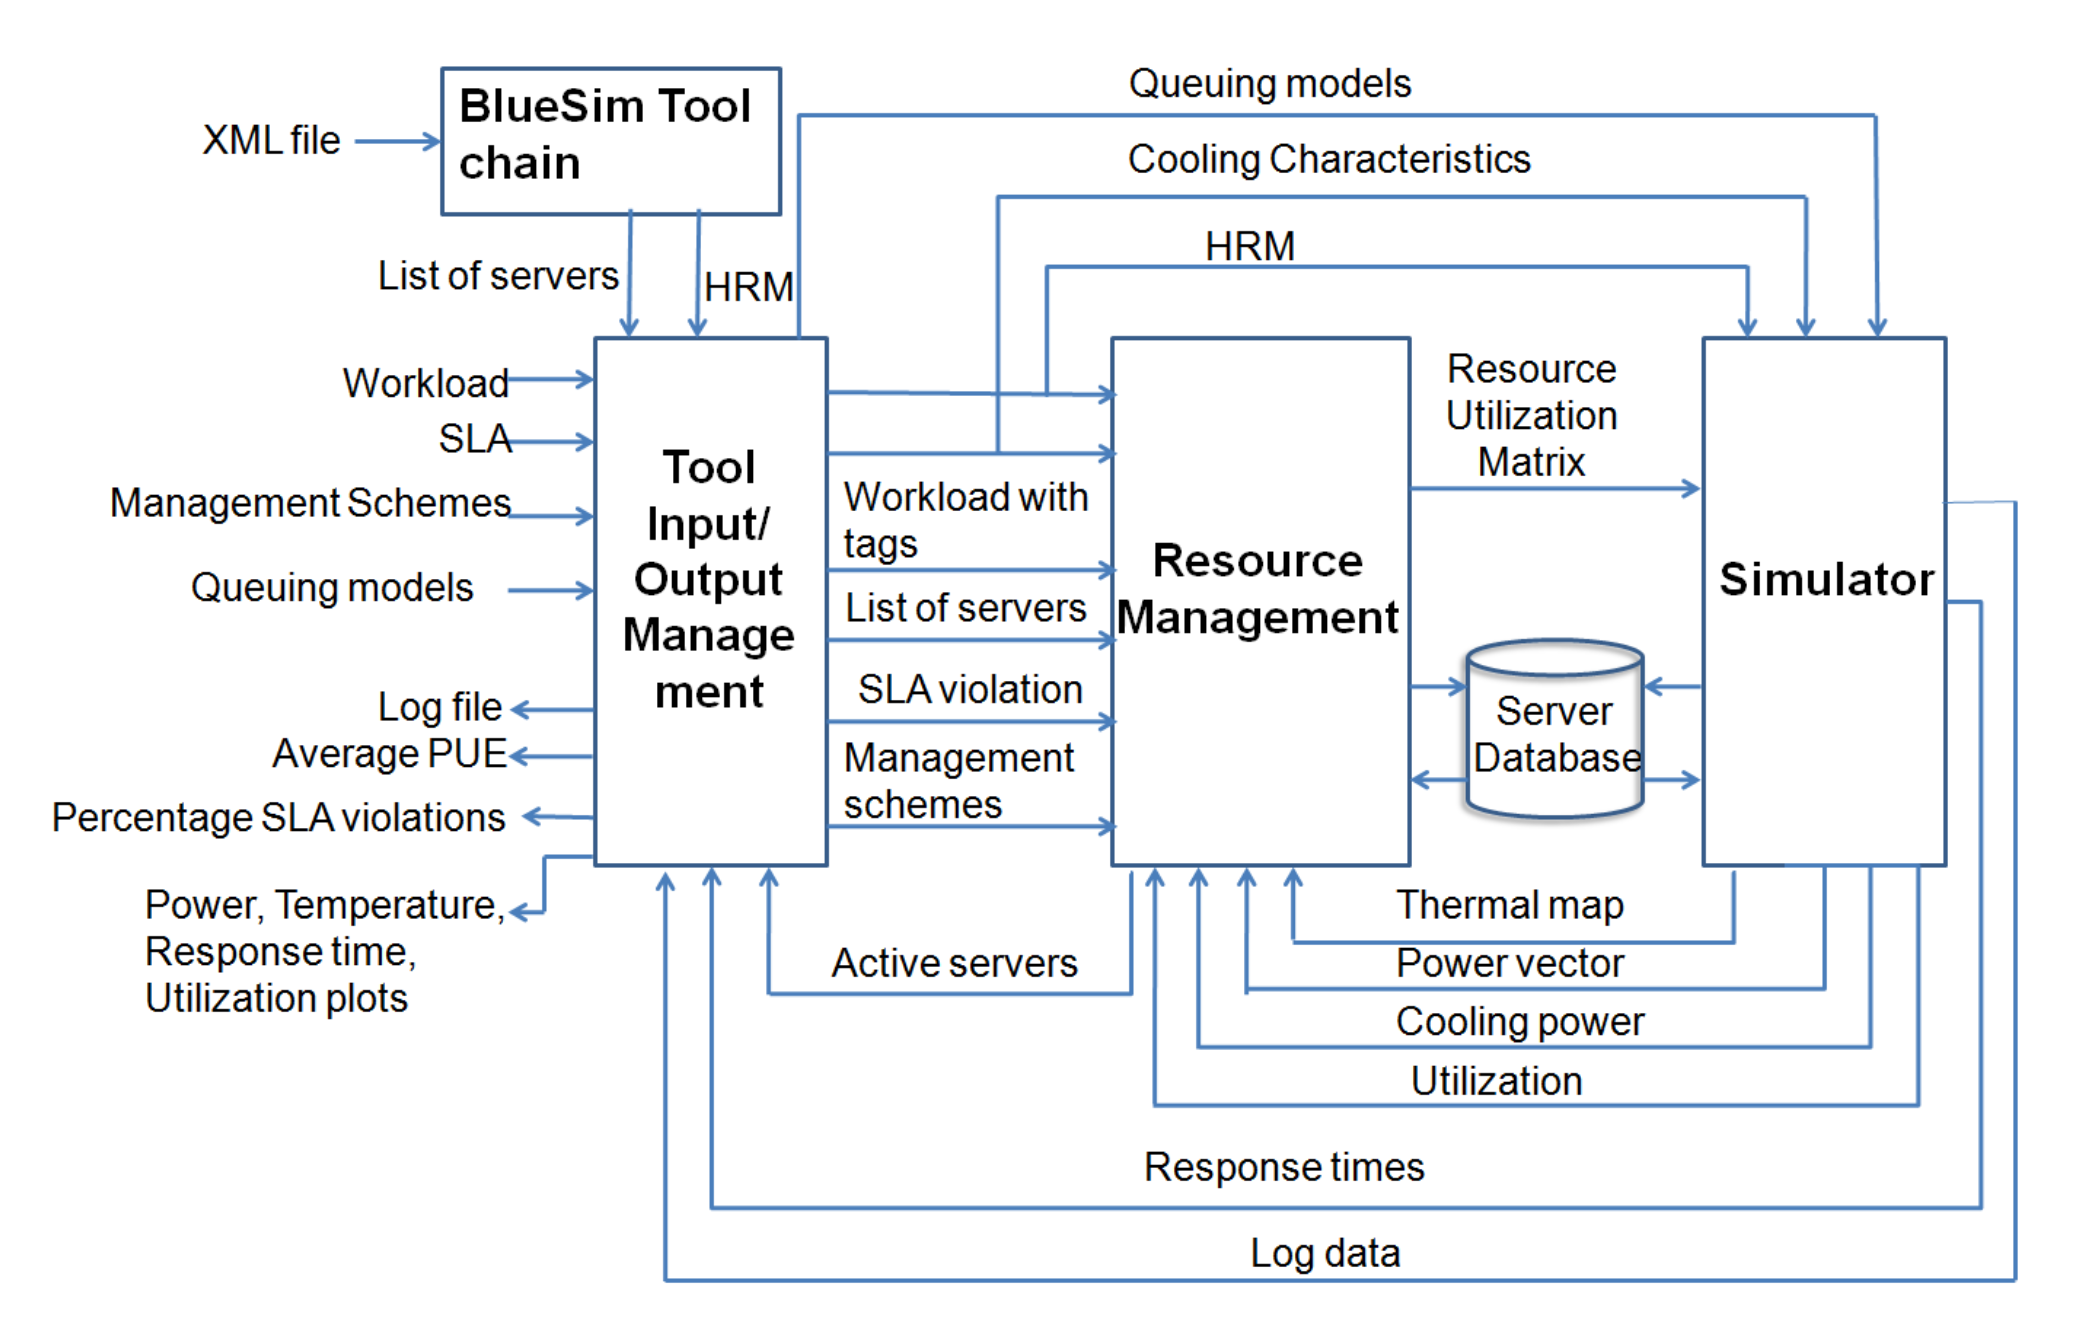
\includegraphics[width=0.5\textwidth]{chapters/images/gdcsim_arch.png}
    \caption{Architecture of the GDCSim simulation environment}
    \label{fig:gdcsim_arch}
\end{figure}

\subsubsection*{CloudNetSim}
\emph{CloudNetSim} \cite{cucinotta2013cloudnetsim} models end-to-end communication between clients and servers. Its extensibility and modularity make it possible to integrate different modules and evaluate different VM deployment algorithms. This simulator provides a platform that allows developers to investigate resource management for realistic cloud applications. However, \emph{CloudNetSim} implements a poor energy and thermal model that makes energy management algorithms implementation difficult. \cite{mansouri2020cloud}
\subsubsection{CloudNetSim++}
\emph{CloudNetSim++} \cite{malik2014cloudnetsim++} is an open source simulator built on the top of \emph{OMNET++}, written in \emph{C++}. It introduces the concept of distributed data centers connected with physical network through various topologies. This simulation tool has a modular architecture that allows researchers to explore different aspects of data centers and to extend network topology by adding switches at the aggregation and core levels. \emph{CloudNetSim++} provides a platform to analyze energy consumption during the simulation and an energy-aware scheduler which supplies several techniques such as Dynamic Voltage and Frequency Scaling. 
\emph{CloudNetSim++} architecture is shown in figure \ref{fig:cloudnetsim++_arch} and consists of five modules:
\begin{itemize}
    \item \textbf{Pricing Policy Manager}: computes the billing cost for each user request based on the agreement;
    \item \textbf{Cloud Usage Monitor}: analyzes usage patterns;
    \item \textbf{Task Scheduling Selection Module}: determines the scheduling policy;
    \item \textbf{VM Manager}: Determines VM assignments according to the received SLA requests;
    \item \textbf{User Task Scheduler}: receives all incoming user requests and distributes them to the appropriate VMs.
\end{itemize}
\begin{figure}[h]
    \centering
    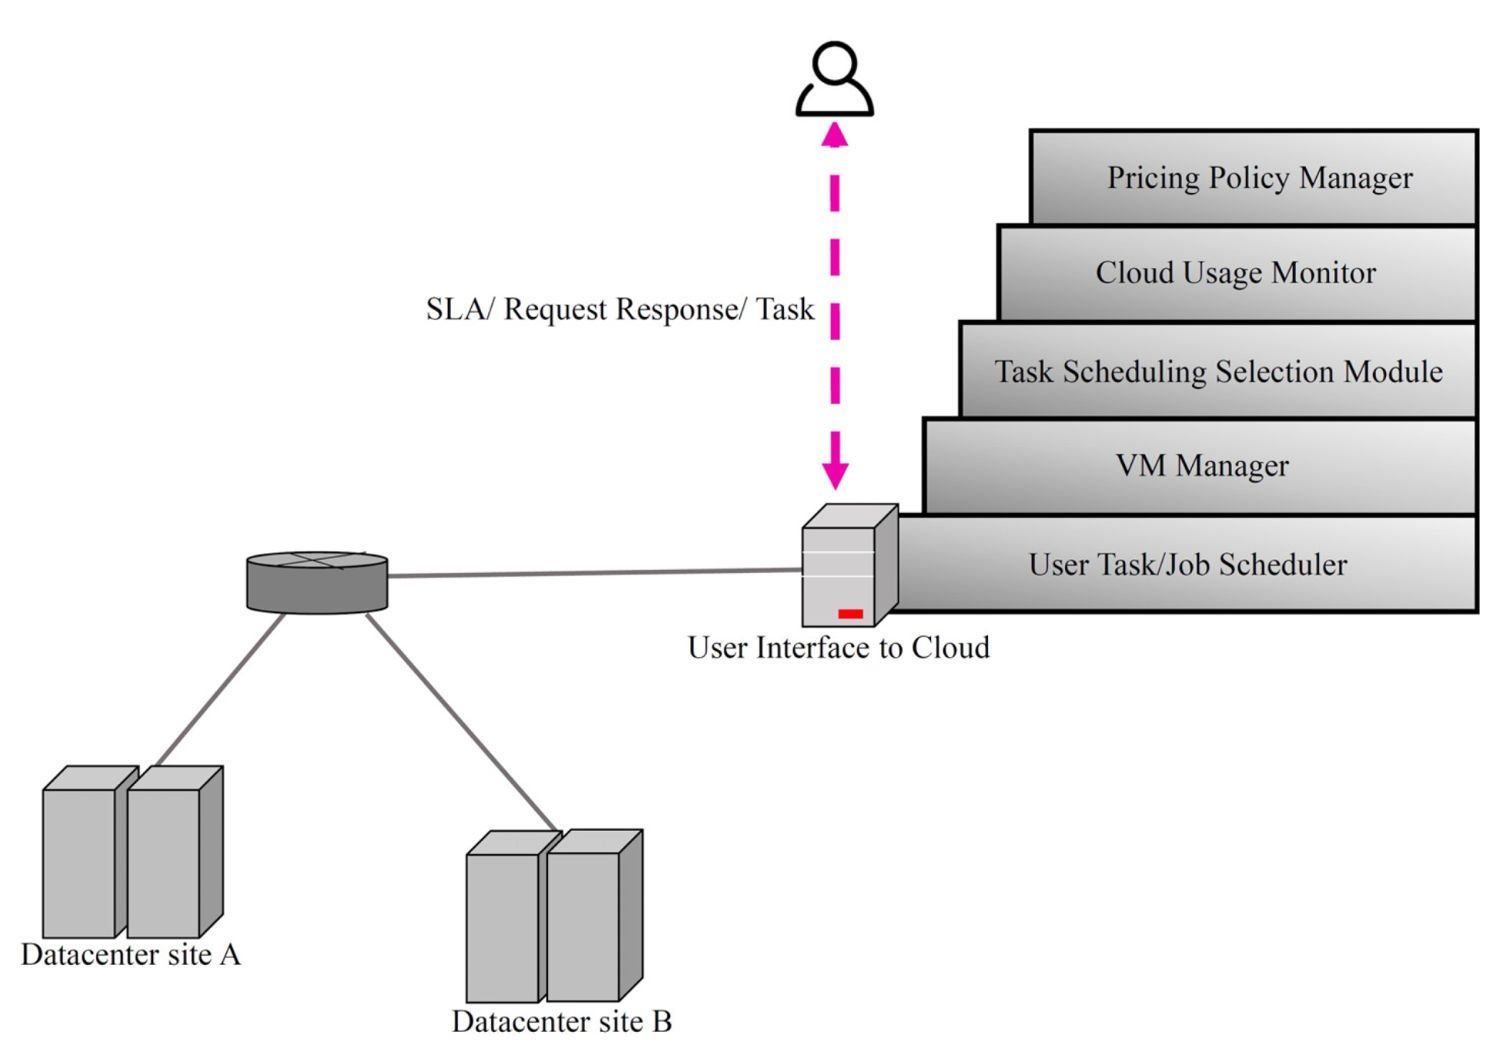
\includegraphics[width=0.5\textwidth]{chapters/images/cloudnetsim++_arch.png}
    \caption{Architecture of the CloudNetSim++ simulation environment}
    \label{fig:cloudnetsim++_arch}
\end{figure}
\subsubsection*{GreenCloud}
\emph{GreenCloud} \cite{kliazovich2012greencloud} is an open source simulator, written in \emph{C++} and \emph{OTcl} and built on the top of \emph{NS2} that enables researchers to study the energy consumption of data centers. \emph{GreenCloud} operates at packet level, as it simulates the behavior of individual network packets and their interactions within the TCP/IP protocol suite that is fully implemented by this simulator. \emph{GreenCloud} aims to provide insights into the energy usage of various components within a data center, including servers, switches, and network links and allows users to evaluate the effectiveness of different energy-saving techniques and algorithms, by accurately modeling the energy consumption models. However, despite its utility in energy monitoring, \emph{GreenCloud} has encountered challenges related to scalability because simulation times in \emph{GreenCloud} tend to be relatively long. This simulator also requires significant memory resources, which can pose constraints on the size and complexity of the simulated scenarios. These scalability limitations can make it difficult to analyze large-scale data center networks or evaluate energy-efficient protocols and algorithms in a timely manner. \cite{mansouri2020cloud}
The structure of \emph{GreenCloud} simulation environment mapped onto the three-tier data center architecture is shown in figure \ref{fig:greencloud_arch}. 
\begin{figure}[h]
    \centering
    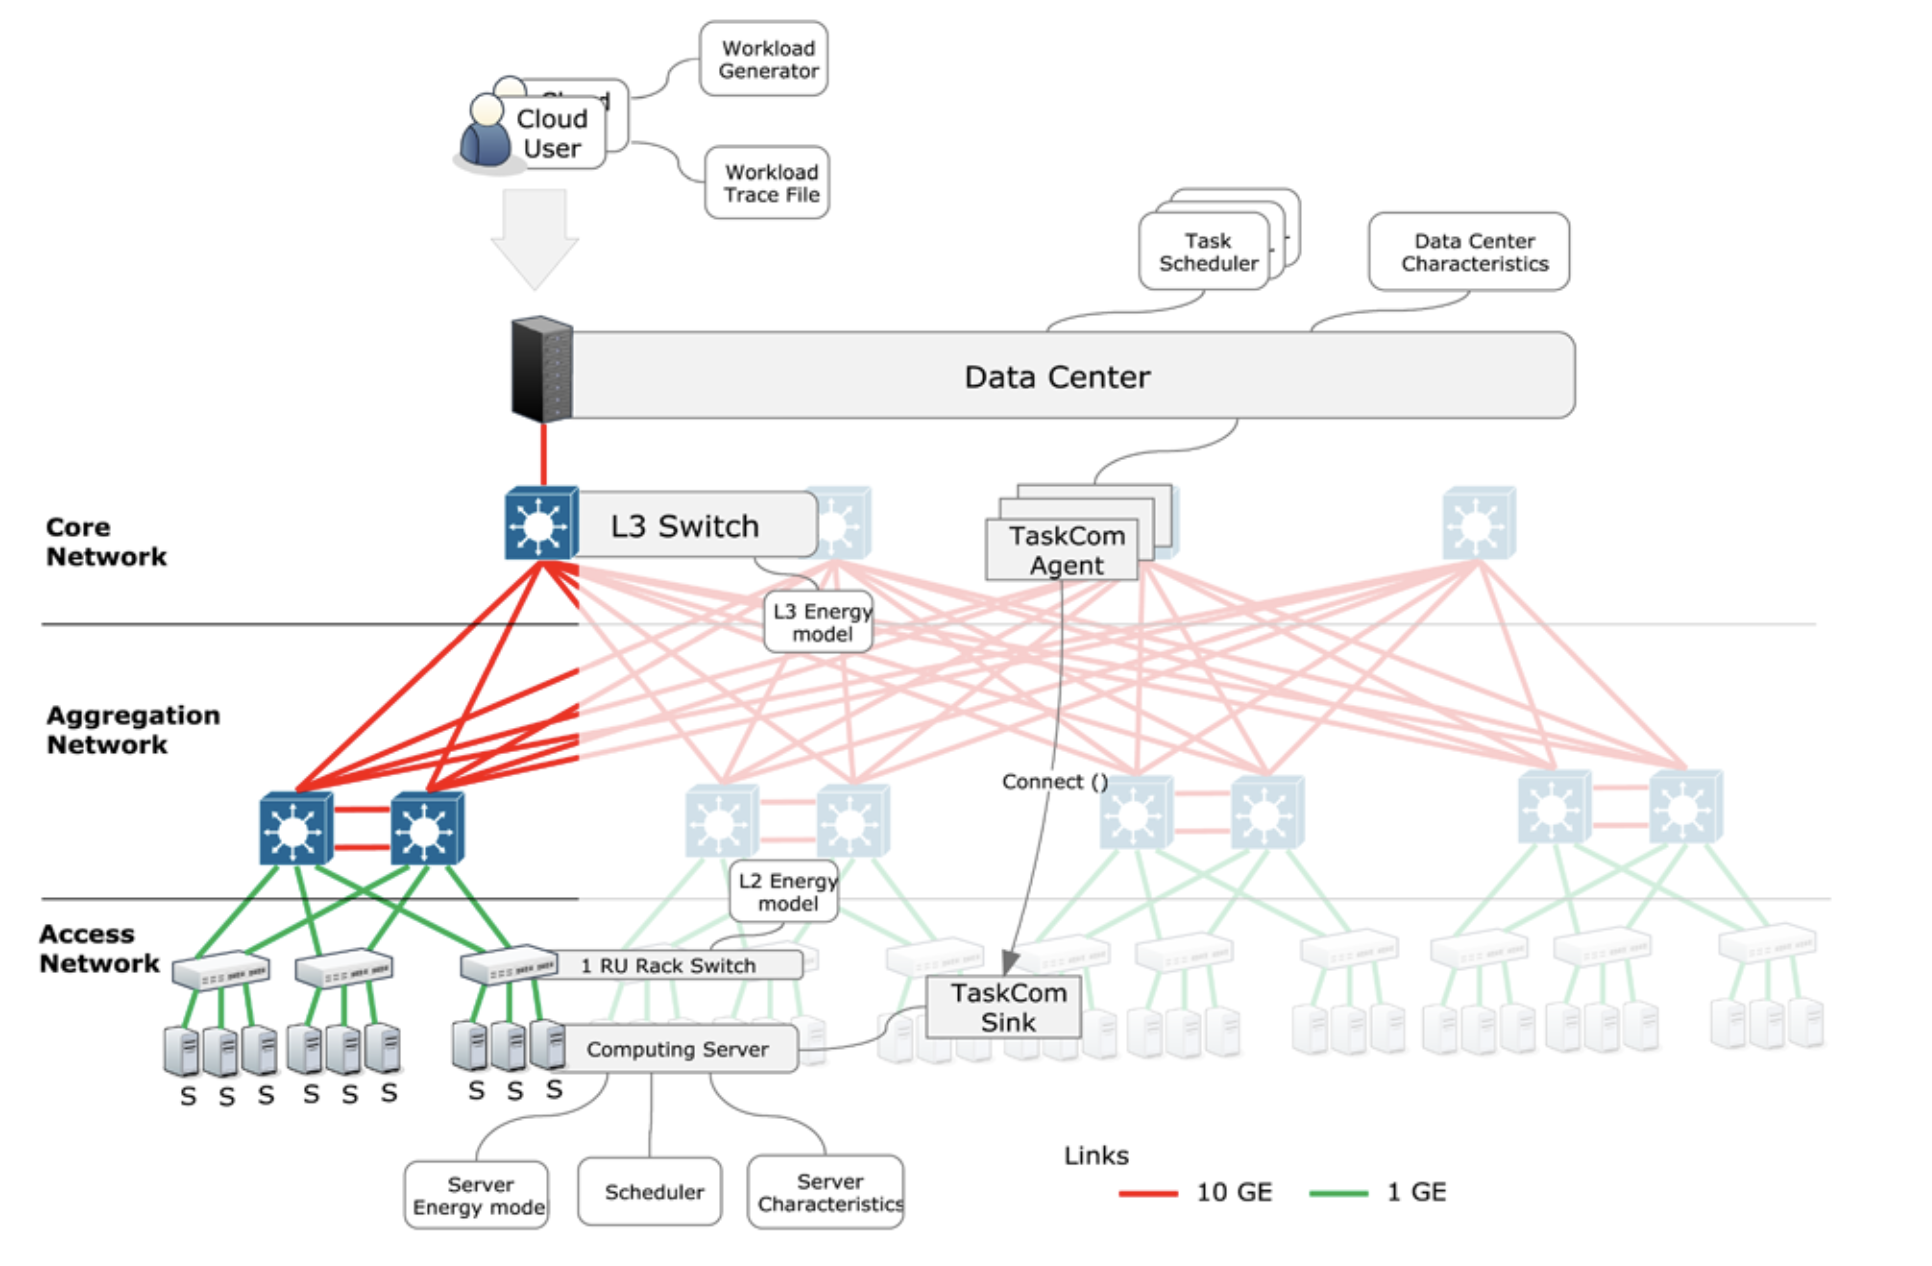
\includegraphics[width=0.5\textwidth]{chapters/images/greencloud_arch.png}
    \caption{Architecture of the GreenCloud simulation environment}
    \label{fig:greencloud_arch}
\end{figure}
\subsubsection*{iCanCloud}
\emph{iCanCloud} \cite{nunez2012icancloud} offers a dedicated \emph{GUI} that allows users to configure the computing center and obtain graphical reports. \emph{iCanCloud} supports the implementation of various brokering strategies, providing the flexibility to define different brokers connecting users and the computing center. However, this simulator does not address aspects related to the energy model and security \cite{mansouri2020cloud}.
\subsubsection*{secCloudSim}
\emph{secCloudSim} \cite{rehman2014seccloudsim} is an extension of \emph{iCanCloud} that implements simple security mechanisms lacking in its predecessor. Among the various security features, it includes an authentication protocol and \emph{Access Control List (ACL)} that allows associating specific privileges with each authenticated user. \emph{secCloudSim} provides a framework where researchers can develop security characteristics such as encryption, decryption, encapsulation, authentication, and privacy. However, the security mechanisms provided by \emph{secCloudSim} are not very advanced, limiting researchers from studying infrastructure vulnerabilities \cite{mansouri2020cloud}.
\subsubsection*{GroudSim}
\emph{GroudSim} \cite{ostermann2011groudsim} is a \emph{Java-based} simulator primarily used in the context of scientific applications. Developers can import \emph{ASKALON} experiments \cite{fahringer2005askalon} into this simulator to conduct simulations of real applications. However, this simulator lacks realism as it does not allow the configuration of a realistic network topology and does not scale effectively \cite{mansouri2020cloud}.

\subsubsection*{CloudSched}
\emph{CloudSched} \cite{tian2013toolkit} implements various energy-efficient algorithms and resource scheduling strategies for physical and virtual machines to avoid bottlenecks. It allows developers to define custom resource scheduling algorithms as needed. However, \emph{CloudSched} does not consider task failures, making it unable to implement fault-tolerance strategies \cite{mansouri2020cloud}.

\subsubsection*{SimIC}
\emph{SimIC} \cite{sotiriadis2013simic} focuses mainly on the heterogeneity of environments in which experiments are executed. Developers can define inter-cloud scheduling algorithms based on various distributed parameters. However, the main limitations of this simulator are that it does not allow investigation of energy consumption, traffic controls, and congestions \cite{mansouri2020cloud}.
\subsubsection*{SPECI}
\emph{SPECI} \cite{sriram2009speci} models aspects related to the scalability and performance of computing centers, allowing developers to monitor the system's behavior by varying its architecture. The simulator also enables investigation of inconsistencies that may arise in the event of failures. However, it does not model changes in the performance of virtual machines during execution, despite this factor being particularly relevant in real-world scenarios \cite{mansouri2020cloud}.

\subsubsection*{SCORE}
\emph{SCORE} \cite{fernandez2018score} is well-suited for defining energy-aware scheduling algorithms, such as mechanisms for shutting down and powering on resources. However, it lacks a security module that would allow developers to investigate fundamental aspects of the computing center related to security \cite{mansouri2020cloud}.


\subsubsection*{GAME-SCORE}
The GAME-SCORE simulator \cite{fernandez2019game} is an extension of the SCORE simulator written in \emph{Scala}, which uses a combination of discrete-event and multi-agent simulation approaches. Its primary purpose is to simulate energy-efficient IaaS in cloud environments. This simulation tool provides the flexibility to dynamically select energy-efficiency policies from a range of options, allowing for the shutdown of idle machines during runtime. As a practical example, it introduces an algorithm based on the Stackelberg Game that utilizes this capability. However, it's important to note that this simulation tool can accommodate other strategies as well. These strategies can involve the dynamic switching between various energy-efficiency policies and scheduling algorithms. The versatility of this tool enables the implementation of different approaches to optimize energy consumption in simulated environments.
Architecture of GAME-SCORE is shown in figure \ref{fig:gamescore_arch}. It is composed of two modules, described below:
\begin{itemize}
    \item \textbf{Core Simulator Module}: the module responsible for executing the experiments composed of a workload generator, a core engine and a scheduling module;
    \item \textbf{Energy-Efficiency Module}: the module responsible for the implementation of the energy-efficiency policies.
\end{itemize}
It is additionally composed of a special module that implements the Stackelberg Game in order to dynamically switch between energy-efficiency policies. 
\begin{figure}[h]
    \centering
    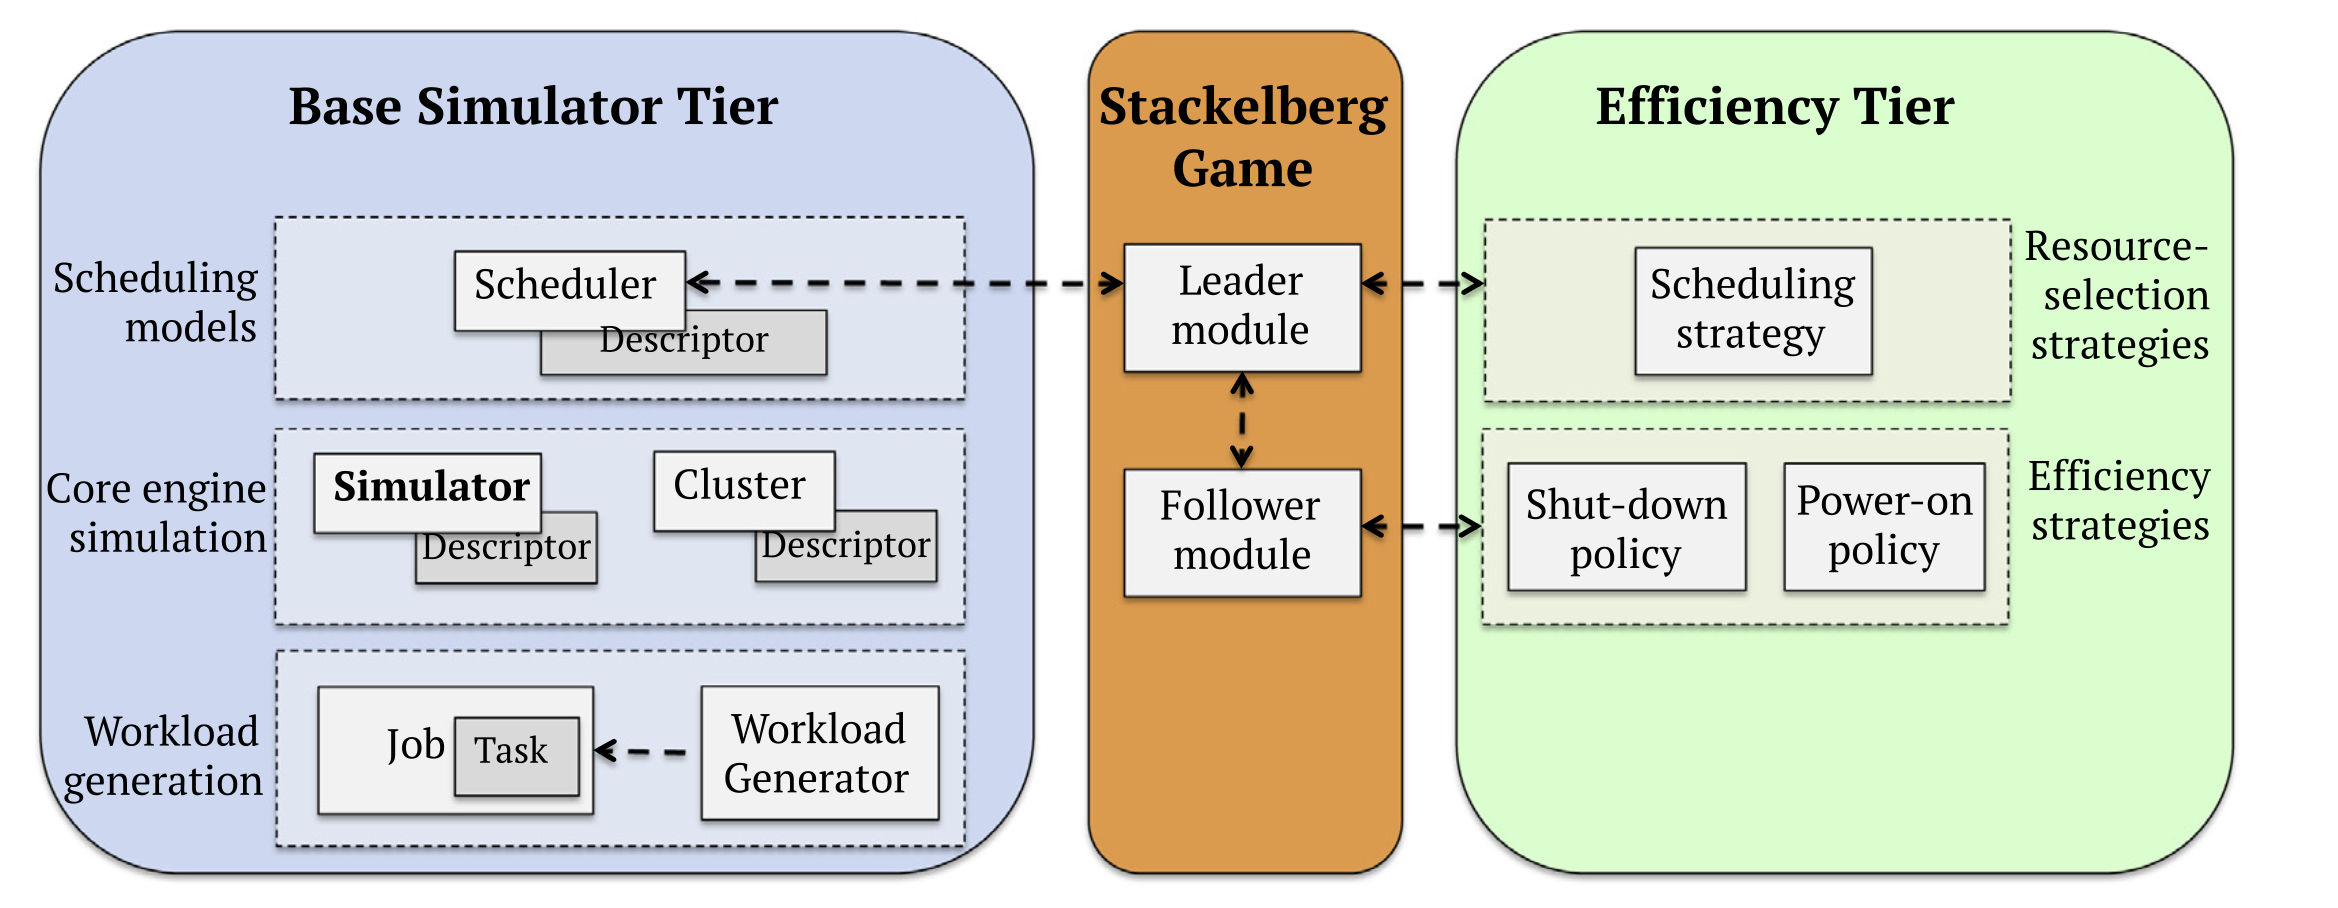
\includegraphics[width=0.5\textwidth]{chapters/images/gamescore_arch.png}
    \caption{GAME-SCORE architecture}
    \label{fig:gamescore_arch}
\end{figure}
\subsubsection*{DISSECT-CF}
\emph{DISSECT-CF} \cite{kecskemeti2015dissect} is an event-based open source simulator written in Java which aims to offer energy-aware scheduling for infrastructure clouds. In contrast to other recently developed simulators, \emph{DISSECT-CF} takes a unique approach by separating energy modeling from resource simulation. This enables the inclusion of energy consumption that may not be directly related to the utilization of data center resources. By decoupling energy modeling, \emph{DISSECT-CF} allows for more comprehensive energy and power modeling, facilitating the analysis of sophisticated energy-aware algorithms in areas such as virtual machine placement and task scheduling. Architecture of \emph{DISSECT-CF} is shown in figure \ref{fig:dissect-cf_arch} and it is composed of five modules decribed below:
\begin{itemize}
    \item \textbf{Event system}: this component serves as the time reference for simulations;
    \item \textbf{Unified resource sharing}: this subsystem establishes a flexible and lightweight foundation for sharing low-level computing resources, such as CPU and I/O;
    \item \textbf{Energy modeling}: \emph{DISSECT-CF} includes components that allow simulator developers to monitor and analyze energy usage patterns of specific simulated resources, such as network links and disks;
    \item \textbf{Infrastructure simulation}: these components govern the behavior and interactions of various elements within the infrastructure, for example the virtual machines;
    \item \textbf{Infrastructure management}: this subsystem offers a user interface, and encompasses higher-level functionalities like virtual machine schedulers of infrastructure clouds.
\end{itemize}
\begin{figure}[h]
    \centering
    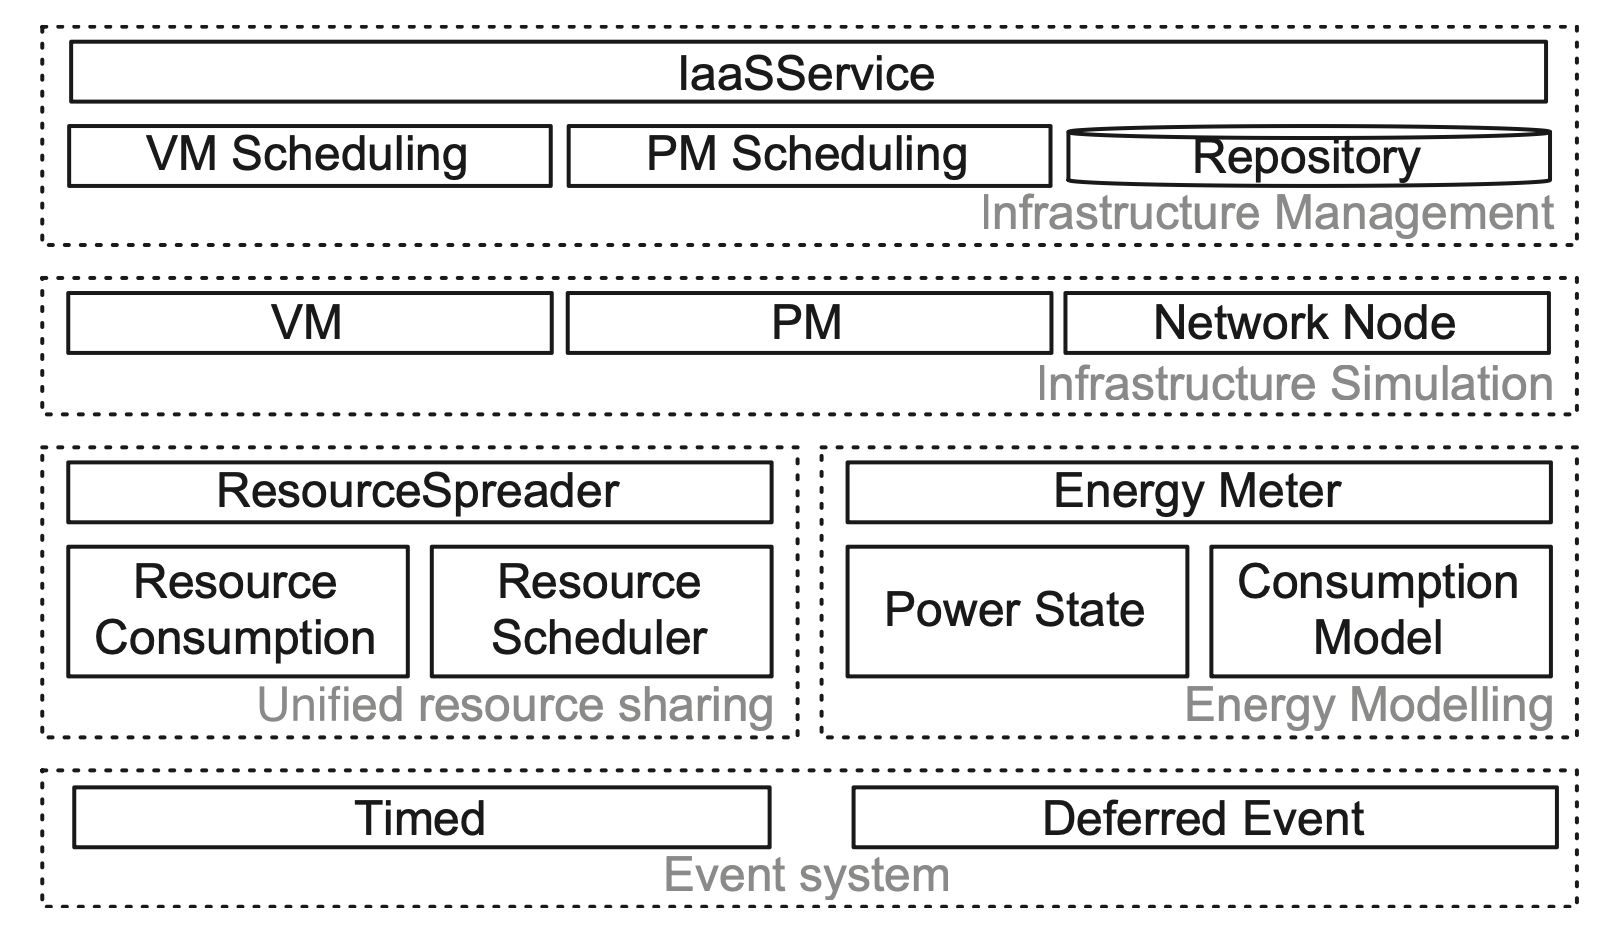
\includegraphics[width=0.5\textwidth]{chapters/images/dissect-cf_arch.png}
    \caption{Architecture of the DISSECT-CF simulation environment}
    \label{fig:dissect-cf_arch}
\end{figure}

\subsubsection{ICARO}
\emph{ICARO} \cite{badii2016icaro} aims to analyze changes in the load of a computing center when the load structure dynamically varies at runtime \cite{khalil2017cloud}.

\subsubsection{SmartSim}
\emph{SmartSim} \cite{shiraz2012extendable} simulates the behavior of mobile devices and resource-intensive applications \cite{khalil2017cloud}. With \emph{SmartSim}, it is possible to model both system components and their behavior in terms of resource allocation and management \cite{suryateja2016comparative}.

\subsubsection{PICS}
\emph{PICS} \cite{kim2015pics} is a simulator designed to evaluate the cost and performance of public IaaS (Infrastructure as a Service) while considering factors related to resource management and job scheduling. However, this simulator lacks a model for communication costs \cite{suryateja2016comparative}.


\section{Choice of simulation tool}
As discussed earlier, this research work requires accurate insights about the energy consumption of the Data Center components. This need led to the selection of the five tools between the ones analyzed in the previous section, that are most focused on analyzing energy consumption, namely: \emph{CloudSim}, \emph{DISSECT-CF}, \emph{GreenCloud}, \emph{GDCSim} and \emph{GAME-SCORE}.
Table \ref{tab:comparison} shows a summary of the selected simulators. As it can be observed, \emph{GDCSim} is stated to be not available. According to the original paper about \emph{GDCSim} \cite{gupta2011gdcsim}, it was mentioned that the simulator would have been available on the \emph{BlueTool} platform once it was ready, however, this platform is no longer accessible. The rest of the information has been gathered from the original papers related to the simulators, namely \cite{son2015cloudsimsdn}, \cite{kecskemeti2015dissect}, \cite{kliazovich2012greencloud}, \cite{gupta2011gdcsim}, \cite{gdcsim_latest} and \cite{fernandez2019game}.
\begin{table}
    \caption{Simulation tools summary}\label{tab:comparison}
    \begin{tabular}{|l|l|l|l|l|l|}
      \hline
      Simulator  & Simulation type             & Language            & Availability  \\
      \hline
      CloudSim   & Event-based                 & Java                & Open source   \\
      DISSECT-CF & Event-based                 & Java                & Open source   \\
      GreenCloud & Packet-level                & C++, oTcl           & Open source   \\
      GDCSim     & Event-based                 & C, C++, Shell       & Not available \\
      GAME-SCORE & Event-based and multi-agent & Scala, Java, Python & Open source   \\
      \hline
    \end{tabular}
\end{table}

\subsection{Comparison parameters}
The selected simulators have been evaluated based on several parameters, including:
\begin{itemize}
    \item \textbf{Last update}: it provides an indication of how well-supported and updated the simulator is; 
    \item \textbf{Popularity}: it gives an idea of how popular the simulator is; 
    \item \textbf{Availability}: it indicates the availability of the simulator;
    \item \textbf{Granularity}: it suggests the level of detail at which the elements of the data center and simulation can be defined; 
    \item \textbf{Performance profile}: it provides an indication of the performance of the simulator;
\end{itemize}

\subsection{Simulators evaluation}
The following sections describe the simulators from the perspective of the evaluation parameters. Each feature of the simulators has been assigned a score on a scale from 1 to 5, in order to highlight strengths and weaknesses. The evaluation results are presented in the radar chart shown in figure \ref{fig:radar}.

\subsubsection{Last update}
\emph{CloudSim}'s, \emph{GAME-SCORE}'s and \emph{DISSECT-CF}'s last update (2020, 2018 and 2023 respectively) were gathered from the latest commits on their GitHub repositories\footnote{CloudSim: https://github.com/Cloudslab/cloudsim,\\ GAME-SCORE: https://github.com/DamianUS/game-score \\ DISSECT-CF: https://github.com/kecskemeti/dissect-cf}. \emph{GreenCloud}'s latest files modification year is 2016 (the project has been download from the simulator platform\footnote{http://greencloud.gforge.uni.lu/ftp/greencloud-v2.1.2.tar.gz}). Since \emph{GDCSim} is not available, we can assume that its last update corresponds to the year of the last paper published about it \cite{gdcsim_latest}, which is 2014.

\subsubsection{Popularity}
Popularity has been evaluated through the citation numbers that have been obtained from the \emph{SCOPUS} platform:
\begin{itemize}
    \item CloudSim: 2043 citations;
    \item DISSECT-CF: 23 citations;
    \item GreenCloud: 31 citations; 
    \item GDCSim: 3 citations;
    \item GAME-SCORE: 1 citation;
\end{itemize}

\subsubsection{Availability}
Tools availability is reported in table \ref{tab:comparison}.

\subsubsection{Granularity}
According to the original papers about the analyzed simulators:
\begin{itemize}
\item \emph{CloudSim} allows to create energy-conscious provisioning policies by overriding the method \emph{getPower()} of the abstract class \emph{PowerModel} whose input parameter is the utilization metric for Cloud host and return parameter is the power consumption value. \emph{CloudSim} also provides a VM Allocation controller component (\emph{VmAllocationPolicy}) that exposes some custom methods which can be used by developers in order to implement new policies based on several optimization goals, and a VM Scheduler component which can be extended to test several allocation policies;
\item \emph{DISSECT-CF} allows developers to define various energy consumption models based on simulation entities' power state. In order to compute energy consumption accurately, this simulator uses several meters and allows developers to define an aggregation function that addresses the dependency between two metered components (e.g., a virtual machine and the physical one where it is hosted);
\item \emph{GreenCloud} fully implements the \emph{TCP/IP} protocol. This simulator is built on top of the \emph{NS2} simulator, allowing customization of network topology and enabling work at the packet-level to implement specific traffic patterns and model real-world scenarios. Furthermore, thanks to its open-source nature, it allows the implementation of various energy management and workload scheduling algorithms;
\item \emph{GDCSim} architecture was designed to be modular and extensible in order to easily plug new components into the simulator and to perform various analysis under different physical configurations. For example \emph{GDCSim} allows to replace the cooling model with a user-defined one and to add new power consumption and resource management models;
\item \emph{GAME-SCORE}'s main aim is to dynamically apply energy policies during simulations by enabling us to dynamically choose between a catalog of energy-efficiency policies that shut-down idle machines in runtime. This simulator allows to implement strategies to dynamically switch between a set of energy efficiency policies and scheduling algorithms during simulations.
\end{itemize}

\subsubsection{Performance profile}
\begin{itemize}
    \item \emph{CloudSim}'s authors conducted various tests in order to analyze the performance. They found out that the time to instantiate an experiment setup with 1 million hosts is around 12 s. Moreover, they observed that the total memory usage never grew beyond 320 MB even for larger system sizes;
    \item \emph{DISSECT-CF}'s authors performed several tests in order to evaluate the performance. In the original paper it was stated that \emph{DISSECT-CF} scales comparably to other state-of-the-art simulators, such as \emph{CloudSim}, since it never drops below linear scaling;
    \item Since \emph{GreenCloud} is a packet-level simulator, its simulation time is significantly higher compared to the other state-of-the-art simulators. Various simulators comparative analysis reported the simulation time as a drawback of \emph{GreenCloud}. In particular \cite{khalil2017cloud} states that \emph{GreenCloud} simulation time is on the order of minutes;
    \item The authors of \emph{GDCSim} conducted several large-scale experiments to validate this simulator. They discovered that each \emph{GDCSim} simulation, which involved \emph{HRM} generation taking 775 minutes, required less than 1 minute to complete. In comparison, corresponding \emph{CFD} simulations took 30 minutes. Therefore, despite the initial cost of generating the \emph{HRM}, \emph{GDCSim} outperforms \emph{CFD} simulations in terms of runtime in the long run \cite{gupta2014gdcsim}.
    \item The authors of \emph{GAME-SCORE} did not provide an insight about their simulator's performance in the original paper \cite{fernandez2019game}. Moreover, none of the previously mentioned works about simulators comparison investigate \emph{GAME-SCORE} performance, so the evaluation of this parameter is not possible. 
\end{itemize}

\begin{figure}[h]
    \centering
    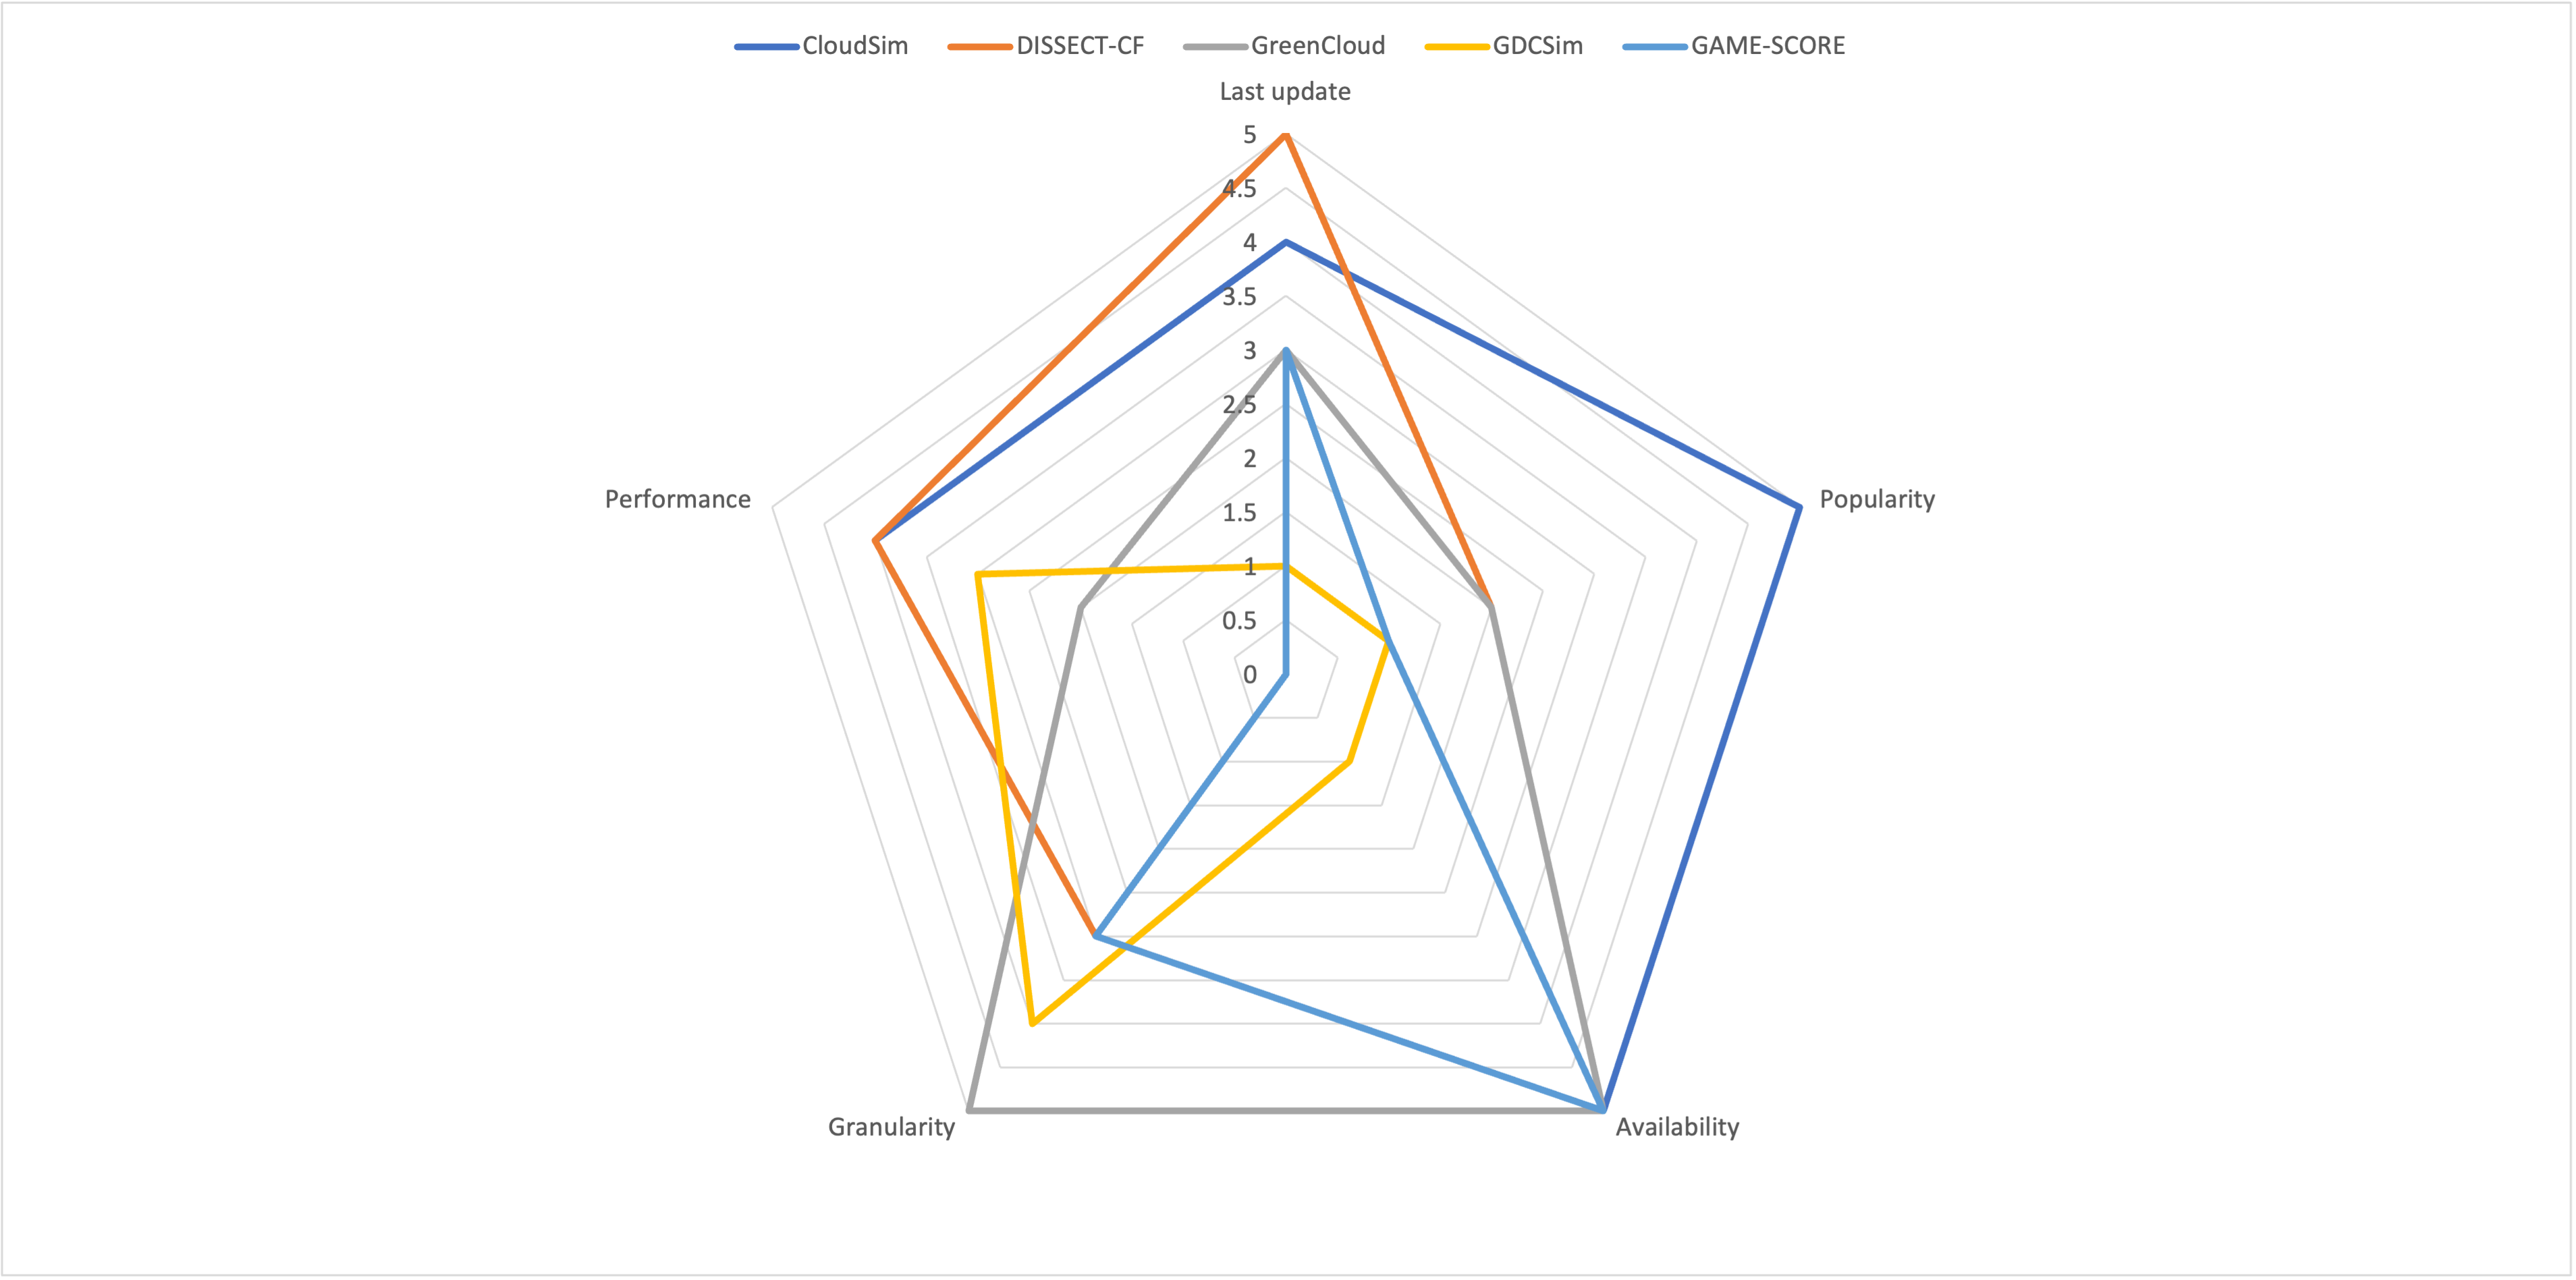
\includegraphics[width=1\textwidth]{chapters/images/simulators_scoring.png}
    \caption{Simulators scoring}
    \label{fig:radar}
\end{figure}

\subsection{Selection of GreenCloud}
Based on the comparisons made among the different analyzed simulators, each of them has its strengths and weaknesses, however, for the needs required in the study addressed by this thesis work, it is essential to prioritize aspects related to the energy consumption of the computing center and the accuracy of simulations. From the conducted comparisons, it is evident that \emph{GreenCloud} is the simulator that accurately considers these aspects as it is built on top of \emph{NS2} simulator and fully implements the \emph{TCP/IP} protocol. Despite \emph{GreenCloud} simulation times tend to be high, for the purposes of this study it is reasonable to prioritize granularity over performance. Therefore, the study will continue using \emph{GreenCloud} as the reference tool for the simulations to be conducted.

}

